\documentclass[11pt]{revtex4-1}
\usepackage[utf8]{inputenc}
\usepackage{physics}
\usepackage{graphicx}
\usepackage{float}
\usepackage{enumitem}
\newenvironment{QandA}{\begin{enumerate}[label=\bfseries\arabic*)]\bfseries}
                      {\end{enumerate}}
\newenvironment{answered}{\par\normalfont}{}

\begin{document}
\section{Questions and answers to the thesis}
	\begin{QandA}
		\item Is there a minimal size of the droplet which host the vortex? No He atom evaporation? (1.2.4 p.11)
		\begin{answered}
			Essentially, yes. For a liquid to support quantum vortices, it needs to be at least in a superfluid state. So the minimal droplet size is dictated by the onset of superfluidity. In $^4$He clusters this was first determined theoretically \cite{Sindzingre89,Pitaevskii90} and confirmed experimentally in Ref.~\cite{Grebenev98} ---where they looked at the infrared spectrum of single oxygen carbon sulfide (OCS) molecules inside helium-4 droplets--- to happen when the cluster size reaches about 60 $^4$He atoms. 

			$^4$He atom evaporation is strongly underestimated in the functional we use, although there are high-energy $^4$He emitted during the dynamics of collisions.
		\end{answered}
	
		\item Is $\lambda_0$ a ratio between an energy from the surface tension and the energy of the dopant-$^4$He interaction? (1.3 p.12)
		\begin{answered}
			Yes, it is defined as
			\begin{align*}
				\lambda\equiv\frac{\rho\,\varepsilon\,r_\mathrm{min}}{\sigma \,2^{1/6}}
			\end{align*}
			where $\varepsilon$ is the well depth of the dopant-$^4$He interaction, $r_\mathrm{min}$ the equilibrium separation, $\sigma$ the surface tension of the droplet and $\rho$ the number density of the droplet. See Ref. \cite{Ancilotto95} for more details.
		\end{answered}
		
		\item When can the SO-coupling be neglected? (2.4.2 p.27)
		\begin{answered}
			That depends on the specific combination of the He-dopant interaction and the SO level splitting of the dopant. Whenever the separation between the energy levels of the He-dopant PECs for the different orbital angular momentum states, \emph{without SO-correction}, are of the same order as the SO level splitting for that dopant, it has to be included. When this is not the case, SO-coupling can be neglected. 	\end{answered}
		
		\item Numerical details: Code parallelised? How? Typical number of points? (p.28)
		\begin{answered}
			I have put these answers and more in the new subsection 2.6.3.
		\end{answered}
		
		\item Chapter 7 too short. A discussion of the current structure of vortex lattices would be welcome, specifically, why is doping important for the detection of vortices. (p.63)
		\begin{answered}
			This has been solved, hopefully, by moving Section 9.5 `\textit{Vortex arrays in $^4$He droplets doped with Ar atoms}' to Section 7.2. I think it fits better in Chapter 7, where it is a nice transition form Section 7.1.
		\end{answered}
		
		\item Other droplet sizes explored compared to Gomez experiments? (8.2 p.66)
		\begin{answered}
			Yes, but not in this thesis. We use $N=5000$ for droplets hosting vortex arrays. This work is being done now, and parts of it will be published this year, specifically the dynamics of cluster formation inside He droplets.
		\end{answered}
		
		\item No SO-orbit in the case of Xe? (8.2 p.66)
		\begin{answered}
			No, because we treat Xe in the ground state $^1$S$_0$.
		\end{answered}
		
		\item He evaporation: are there reflections of these emitted He atoms at the edges of the box? (p.67)
		\begin{answered}
			Normally, yes, because we use periodic boundary conditions for our box, but we took care of that by putting an absorbing potential just before the boundaries of the calculation box. I have included an extra subsection 2.6.3 `Absorbing potential at the box boundaries' where this is explained in more detail.
		\end{answered}
		
		\item Other impact parameters explored? (8.2 p.69)
		\begin{answered}
			Yes, but not in Chapter 8. See Chapter 9.
		\end{answered}
		
		\begin{figure}[!]
			\begin{center}
				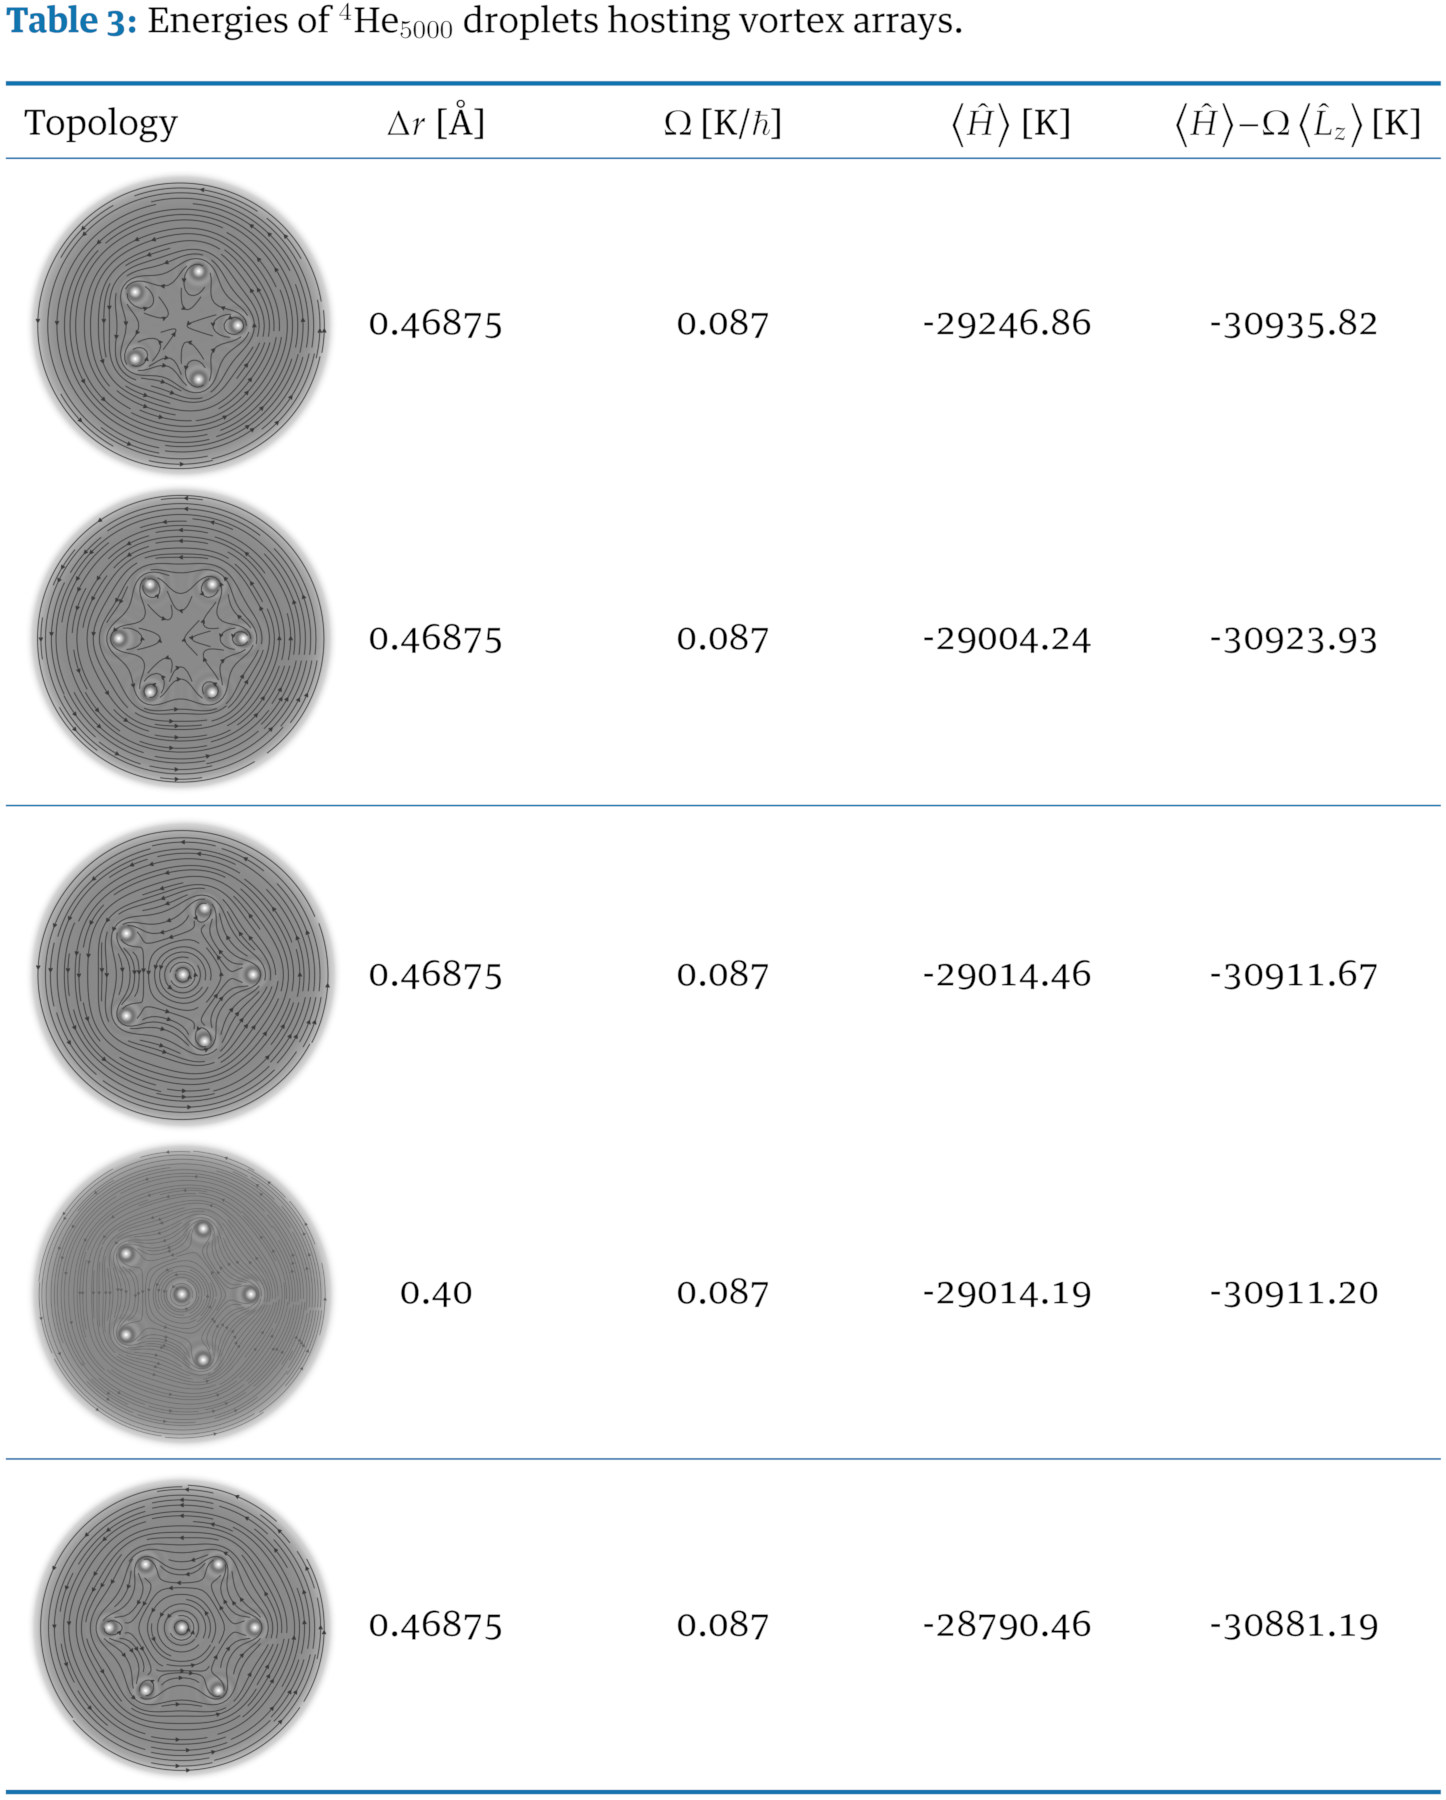
\includegraphics[width=\linewidth]{vortex-energies}
			\end{center}
			\caption{}
		\end{figure}
		
		\item In the vicinity of the impurity, the He not superfluid anymore? How are He I and He II treated in the TDDFT approach? (p.71)
		\begin{answered}
			In our TDDFT formalism at $T=0$ we assume that the whole system is Bose-Einstein condensed, and the parameters of the phenomenological expression for the correlation energy density $\mathcal{E}_\mathrm{c}$ are fitted to reproduce the properties of bulk liquid He II at zero pressure. So, He I is not treated at all.
			
			About the question of superfluidity in the vicinity of impurities; that depends on the strength of the $^4$He-impurity interaction. For example, in Ref.~\citep{Holler2014}, \textit{Superfluidity of helium-4 around a Mg$_{11}$ cluster}, they report that the superfluid fraction in the first solvation shell around the Mg$_{11}$ cluster goes to 100\% for $^4$He$_N$ cluster sizes of $N\sim40$ atoms (see Fig. 6, top panel). This seems to be about 20 atoms less than was determined in Refs.~\citep{Sindzingre89,Pitaevskii90,Grebenev98}. As I understand it so far, it depends on what you are looking at when you want to find signatures of superfluidity. Sindzingre looked at the appearance of the lambda point (it was a PIMC calculation); Grebenev at the ro-vibrational spectrum, and Pitaevskii was also on rotations.
			
			On the other hand, in Refs.~\citep{Kwon12,Shin12} where they did a PIMC study on the fullerenes C$_{20}$ and C$_{60}$ they found that in some cases the local superfluid fraction is completely suppressed for sizes that promote a solid-like order of the $^4$He atoms that is commensurate with the lattice of the fullerene surface.
		\end{answered}
		
		\item Not constant energies. Missing E converted to pot E? (p.80)
		\begin{answered}
			I am not sure what you mean by this question.
		\end{answered}
		
		\item No interaction between vortices? (p.83)
		\begin{answered} 
				Yes, but this is a trial function. After imprinting it is relaxed by the `Imaginary Time Propagation'-method to obtain the real wave function. See Section 2.5.2 for more details.
		\end{answered}
		
		\item Eq.~(9.5) says $\omega_c=0.0167$ (p.83)
		\begin{answered}
			Yes, but Eq.~(9.5) gives the critical value to nucleate 1 linear vortex, the $\omega_c$ on the next page gives the critical value to nucleate 2 linear vortices.
		\end{answered}
		
		\item Does this mean that in experiments and/or model with dissipation you would expect the Xe/Ar be captured in the core? (p.85)
		\begin{answered}
			Yes, static calculations show that the energy is minimised if the impurity is inside the core. Or better, the core will connect to the secondary surface due to the atomic bubble of the impurity, as symmetrically as possible to minimise the energy.
			
			We have been thinking of a way to include some kind of dissipation mechanism in our code in the past but we never got around to actually do it.
		\end{answered}
		
		\item What are the energies of 6 linear vortices in a ring compared to the 6 linear vortices in a ring + 1 linear vortex in the centre? (p.87)
		\begin{answered}
			I didn’t have these numbers at the time of writing since it was francesco who performed the calculations. Because the doctoral school didn't allow an ``article thesis'' anymore, this was mostly a copy/paste from the \LaTeX-source of the already published paper. We therefore decided to leave it as is, while just removing the introduction and method section. Since I have the numbers now I have included them in Fig.1 (Table 3).
		\end{answered}

		\item 200~m/s for Xe is much higher than the 23.7~m/s for Xe in bulk He II as in I.A. Pshenichnyuk and N. G. Berloff, Phys. Rev. B 94, 184505 (2016)? (p.93)
		\begin{answered}
			 We use values that are in the thermal regime of the experiments. Once the droplet's surface is pierced the cruising speed of the Xe atom is lower than the critical Landau velocity (which is about 90~m/s in out functional) in He II. Where did you get this number? I could not find it in the paper. They also seem to use a different model based on Gross-Pitaevskii. In this model the critical Landau velocity is different from ours, but I don't know the value. That could also explain their use of a lower velocity. We did calculations with Xe at 10~m/s starting about 10~\AA{} away from the vortex core to simulate the fate of thermalised solvated Xe atoms in he droplets. They are captured as well.	
		\end{answered}

	\end{QandA}
	
	\begin{thebibliography}{9}	
		\bibitem{Sindzingre89}
			P. Sindzingre, M.L. Klein and D.M. Ceperley,
			Phys.~Rev.~Lett.~\textbf{63}, 1601
			(1989),\\
			doi: https://doi.org/10.1103/PhysRevLett.63.1601

		\bibitem{Pitaevskii90}
			L. Pitaevskii and S. Stringari,
			Z.~Phys.~D~\textbf{16}, 299
			(1990).

		\bibitem{Grebenev98}
			Slava Grebenev, J. Peter Toennies and Andrei F. Vilesov,
			Science~\textbf{279}, 2083--2086
			(1998),\\
			doi: 10.1126/science.279.5359.2083

		\bibitem{Ancilotto95}
			F. Ancilotto, P.B. Lerner and M.W. Cole,
			J~Low~Temp~Phys~\textbf{101}, 1123
			(1995),\\
			doi: https://doi.org/10.1007/BF00754527

		\bibitem{Holler2014}
			J. Höller, E. Krotscheck and R.E. Zillich,
			Eur. Phys. J. D~\textbf{68}, 372
			(2014)
		
		\bibitem{Kwon12}
			Y. Kwon and H. Shin,
			Phys. Rev. B \textbf{82}, 172506
			(2010)
			
		\bibitem{Shin12}
			H. Shin, Y. Kwon,
			J. Chem. Phys. \textbf{136}, 064514
			(2012) 
	\end{thebibliography}
	
\end{document}